\chapter{界面设计}
\section{客户端界面}
% 此处应当有一个简略的图,重点是展示你与用户交互的逻辑。(processon上画一个不花时间)
\begin{figure}[h]
	\centering
	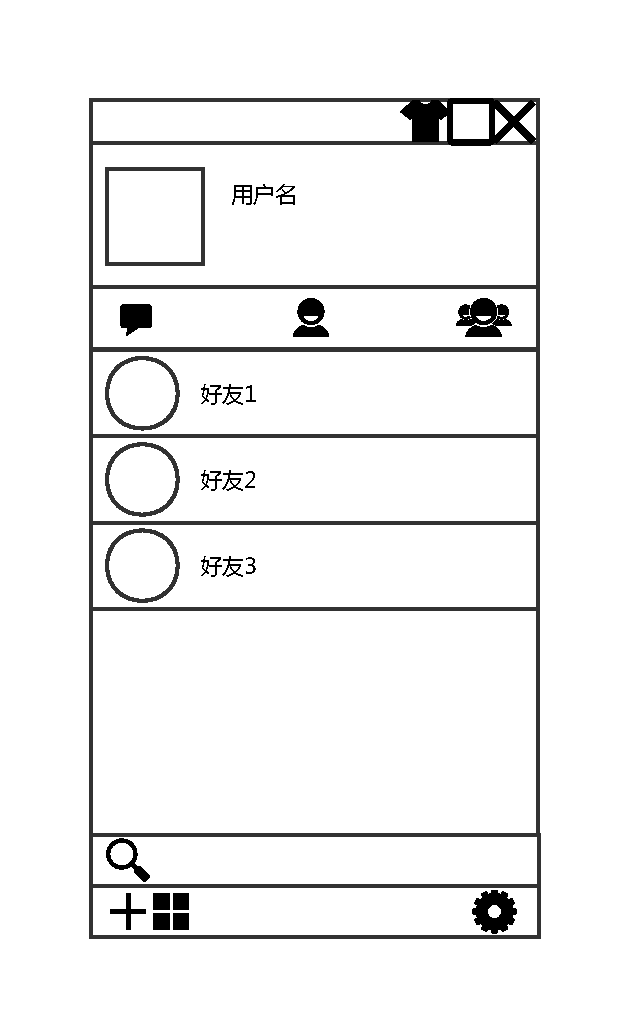
\includegraphics[width=10cm]{main_ui}
	\caption{主界面} \label{fig:main_ui}
\end{figure}


最上方显示自己的头像和用户名。
中间有三个标签页,从左到右分别是会话,好友和群组。
下方有一个搜索框,可用于搜索已添加的好友。
最下方的三个按钮的功能分别是添加新好友,菜单和设置。

见图-\ref{fig:main_ui}

\begin{figure}[h]
	\centering
	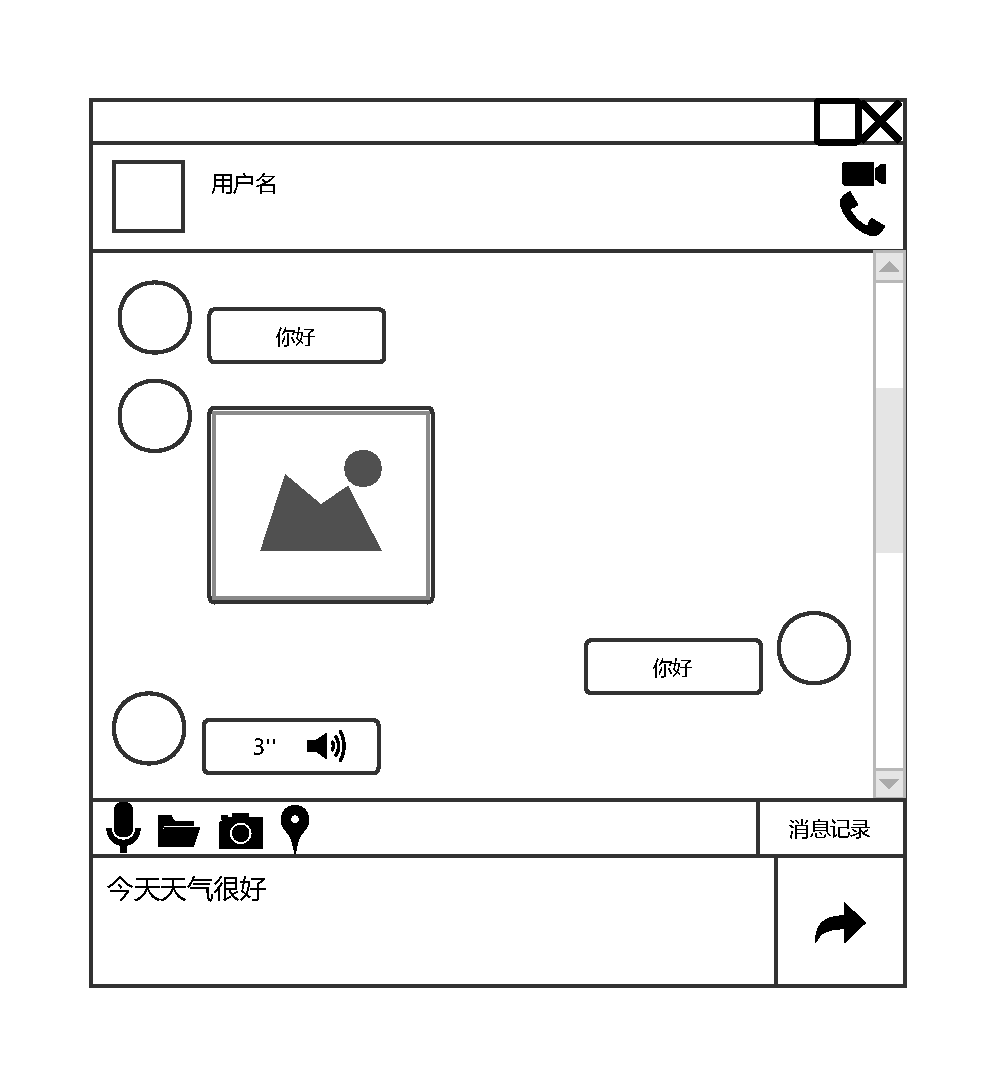
\includegraphics[width=10cm]{chat_ui}
	\caption{聊天界面} \label{fig:chat_ui}
\end{figure}


最上方显示对方的头像和用户名(或群的头像和群名),左侧可以开启视频或语音聊天。
中间为消息显示区,消息放在气泡中显示,自己的消息在右侧,其他人的在左侧。
最下方为文本输入框,左侧为发送按钮。
输入框上方为工具栏,可以用于发送图片和语音消息,可以查看聊天记录。

见图-\ref{fig:chat_ui}

\section{服务器端界面}
% 此处应当有一个简略的图。

\begin{figure}[h]
	\centering
	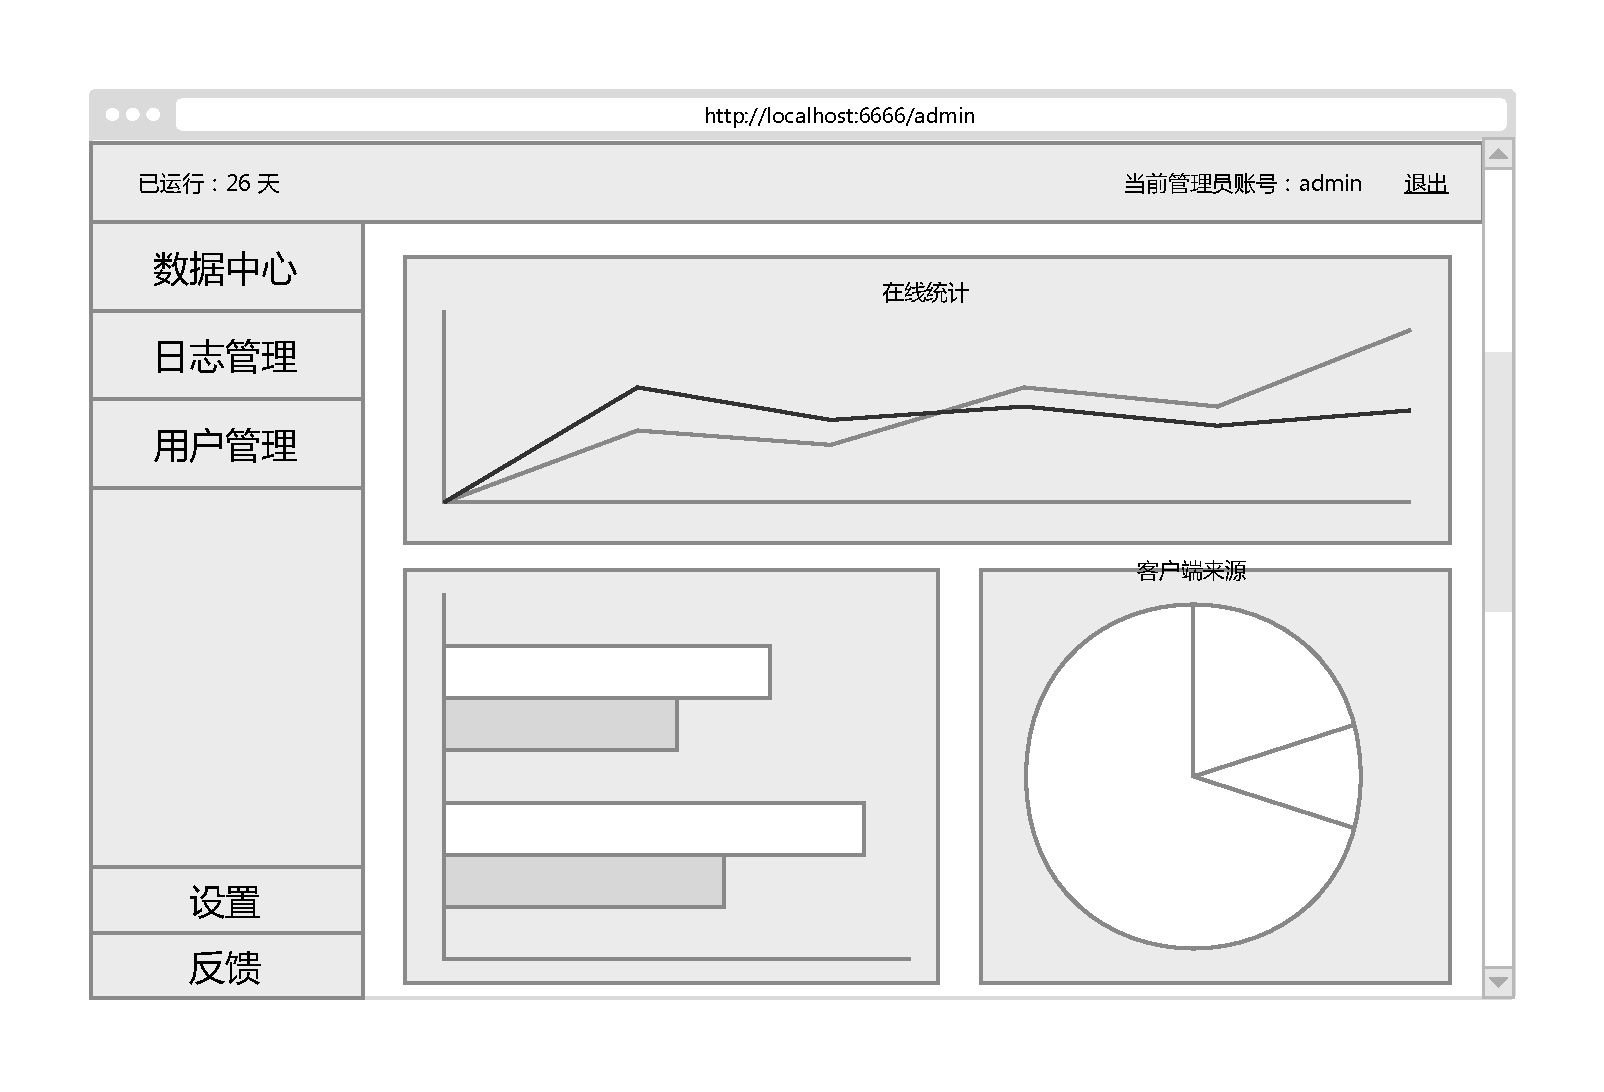
\includegraphics[width=13cm]{admin_ui}
	\caption{服务器端界面} \label{fig:admin_ui}
\end{figure}

服务端提供一个web管理接口,管理员可以通过浏览器打开。
web接口提供日志查看,数据统计,账号管理等功能。

见图-\ref{fig:admin_ui}


\section{登录界面}
% 此处应当有一个简略的图。

\begin{figure}[h]
	\centering
	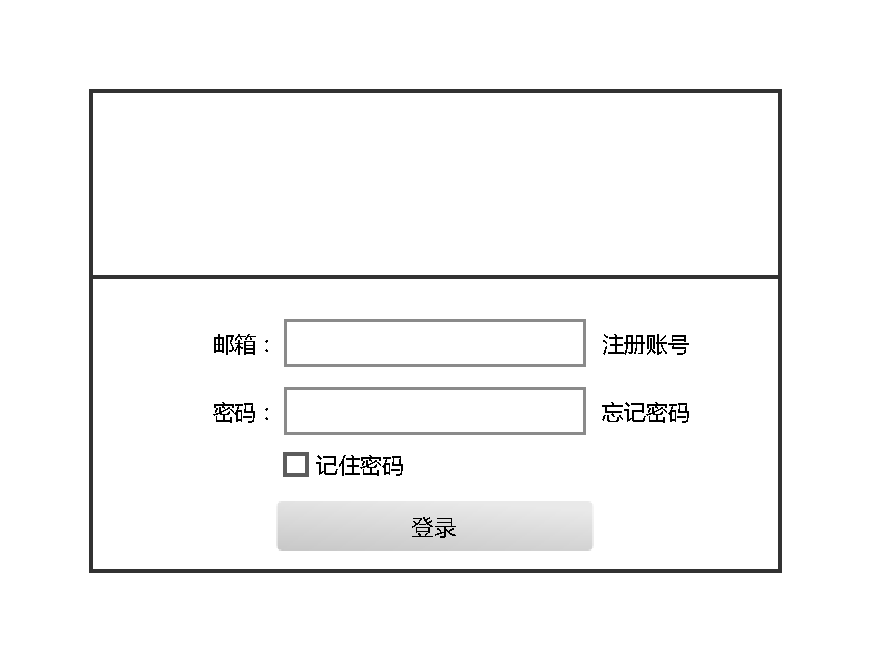
\includegraphics[width=13cm]{login_ui}
	\caption{登录界面} \label{fig:login_ui}
\end{figure}

输入邮箱密码登陆,可选择记住密码,右侧有注册账号和忘记密码的按钮。
界面上方放置banner图片,增加美观。

见图-\ref{fig:login_ui}


\section{用户搜索功能界面}
\begin{figure}[h]
	\centering
	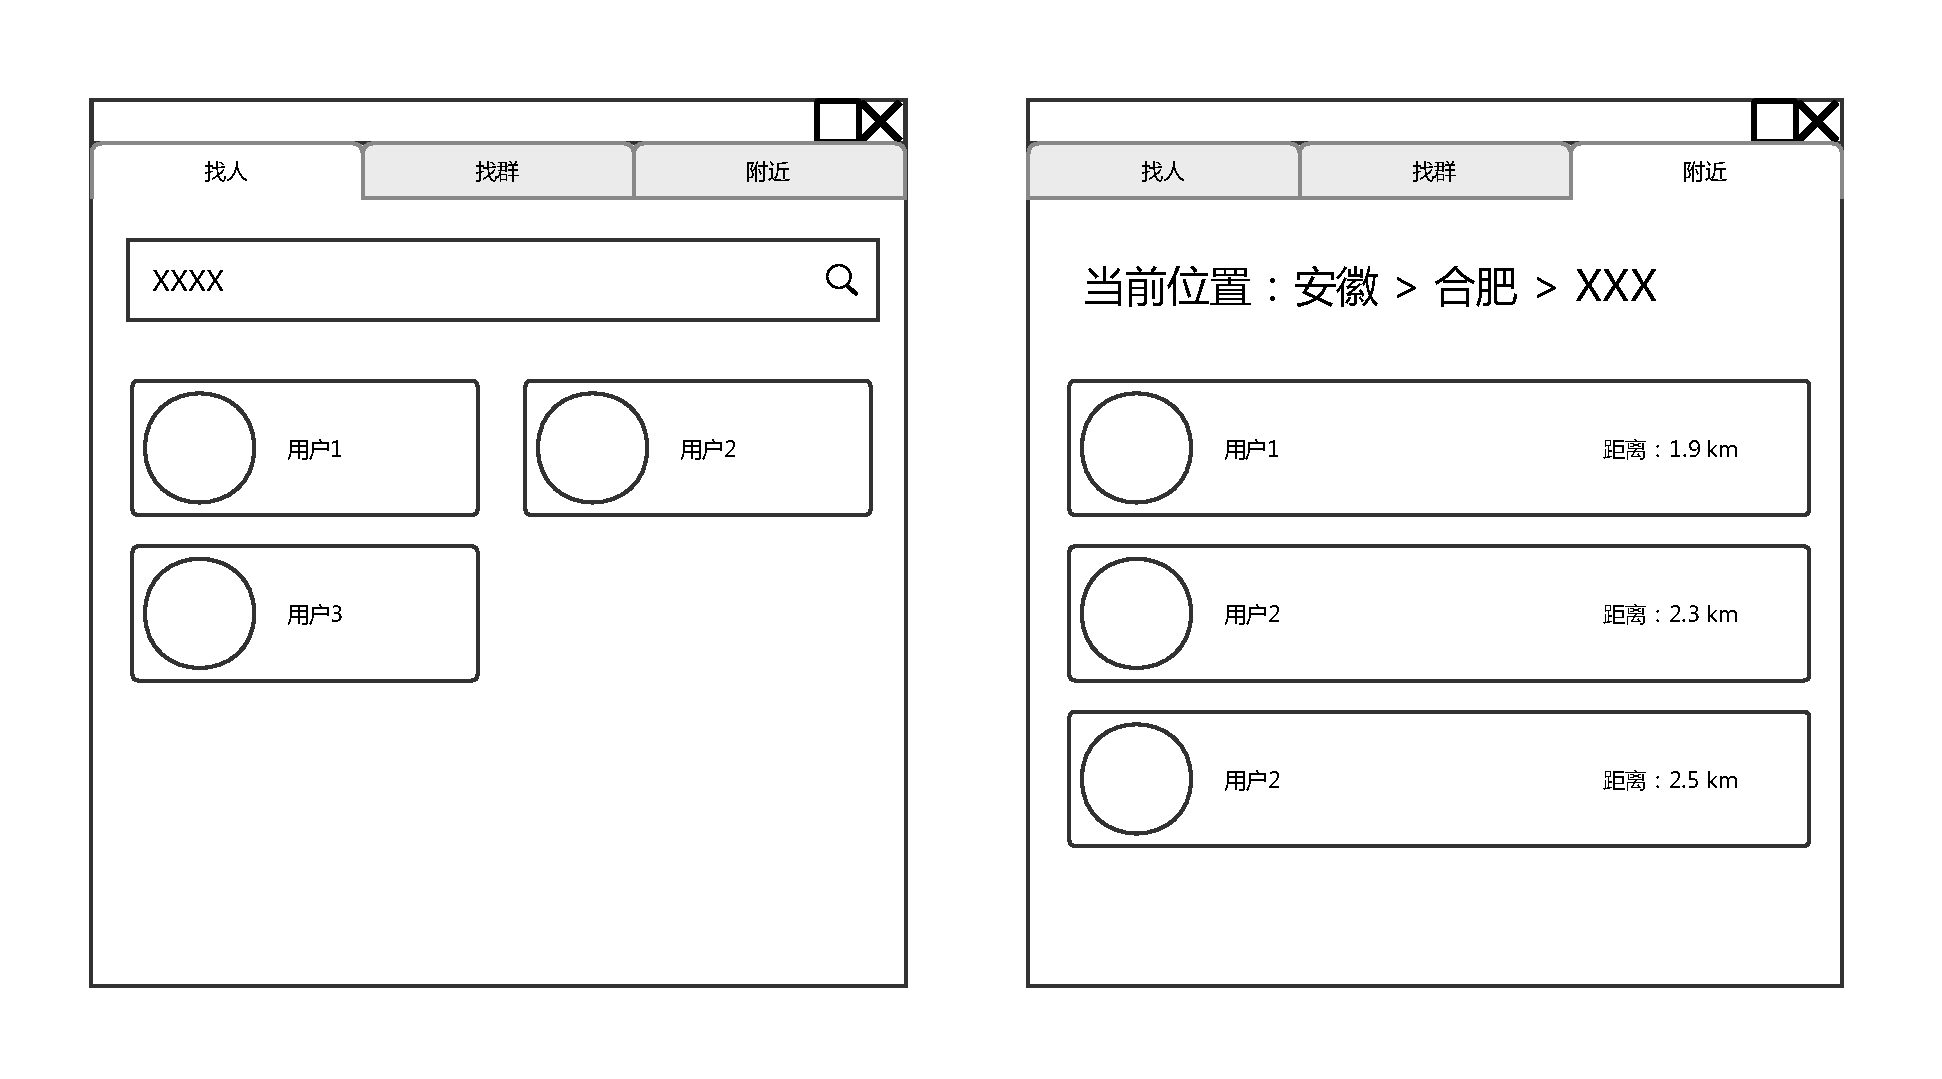
\includegraphics[width=15cm]{search_friend_ui}
	\caption{用户搜索界面} \label{fig:search_friend_ui}
\end{figure}

共三个标签页可用于搜人,搜群,附近。
找人,找群标签页在搜索框输入内容后显示结果。
附近标签页显示了当前位置和附近的用户以及估计的距离。
点击用户弹出用户信息界面。

见图-\ref{fig:search_friend_ui}
